\documentclass[11pt]{beamer} % Определяем тип документа как презентацию
% в квадратных скобках размер шрифта: 8pt, 9, 10, 11 (def), 12, 14, 17, 20.

\input{preamble} 
% В преамбуле можно сделать небольшие изменения (цвет, шрифт итд.) Если есть желание изменить больше, возможно, проще выбрать другой шаблон.

%Логотип
\titlegraphic{\includegraphics[height=1.9cm]{images/mipt_logo.png}}

%Размеры шрифтов титульного листа; Цвета определены в преамбуле
\setbeamerfont{title}{size=\huge}
\setbeamerfont{subtitle}{size=\large}
\setbeamerfont{author}{size=\normalsize}
\setbeamerfont{date}{size=\normalsize}
\setbeamerfont{institute}{size=\normalsize}
% Больше о шрифтах вы найдете в том числе по следующей ссылке:
% https://tex.stackexchange.com/questions/183052/what-are-all-the-possible-first-arguments-to-setbeamerfont

%Тут квадратные скобки --- всё, что будет внизу странички
\title[ФРКТ, МФТИ]{Работа 4.3.1}
\subtitle{Изучение дифракции света}
\author[Тихонов Д.Р., Казачков А.Н.]{}
\institute[]{Московский физико-технический институт \\ Физтех-школа Радиотехники и Компьютерных Технологий}
\date[\textcolor{white}{19 февраля 2024 г.}]{19 февраля 2024 г.}



% Следующее пригодится, если нужно показывать начало секции с оглавлением
%\AtBeginSection[]
%{
%  \begin{frame}
%    \frametitle{Contents}
%    \tableofcontents[currentsection]
%  \end{frame}
%}

% \AtBeginSection[]{
%   \begin{frame}
%   \vfill
%   \centering
%   \begin{beamercolorbox}[sep=8pt,center,shadow=true,rounded=true]{title}
%     \usebeamerfont{title}\insertsectionhead\par%
%   \end{beamercolorbox}
%   \vfill
%   \end{frame}
% }

\addto\captionsenglish{\renewcommand{\figurename}{Рисунок}}

\begin{document}

\frame{\titlepage}

\begin{frame}
    \frametitle{Содержание работы}
    \tableofcontents
\end{frame}

% % Далее начнем работу со слайдами:
\section{Цели работы}
    \begin{frame}{Цели работы}
        \begin{itemize}
            \item исследовать явления дифракции Френеля и Фраунгофера на щели
            \item изучить влияние дифракции на разрешающую способность оптических инструментов
        \end{itemize}
    \end{frame}

    \section{Оборудование}
    \begin{frame}{Оборудование}
        \begin{itemize}
            \item оптическая скамья
            \item ртутная лампа
            \item светофильтр
            \item щели с регулируемой шириной
            \item рамка с вертикальной нитью
            \item экран с двойной щелью
            \item микроскоп на поперечных салазках с микрометрическим винтом
            \item зрительная труба
        \end{itemize}
    \end{frame}

    \section{Дифракция Френеля} 

    \begin{frame}{Теория. Основные понятия}
        \textbf{Дифракция} -- отклонения в распространении волн от законов геометрической оптики. \\
        Основные параметры дифракции: $\boldsymbol{\lambda}$ -- длина волны, $\boldsymbol{b}$ -- размер отверстия, $\boldsymbol{z}$ -- расстояние до плоскости наблюдения. \\
        Характер дифракционных явлений определяется значением \textbf{волнового параметра}
        \begin{equation}
            p = \frac{\sqrt{\lambda z}}{b}.
        \end{equation}
        \begin{itemize}
            \item если $p \gg 1$ -- область дифракции Фраунгофера (\textit{дальняя волновая зона})
            \item если $p \sim 1$ -- область дифракции Френеля (\textit{ближняя волновая зона})
        \end{itemize}
    \end{frame}

    \begin{frame}{Теория. Граничное поле}
        \begin{columns}
            \column{0.5\textwidth}
            \begin{figure}[H]
            \centering
                \includegraphics[width = \textwidth]{images/theory_boundary_field.jpg}
                \caption{Произвольный тонкий экран}
            \end{figure}

            \column{0.5\textwidth}
                Для произвольного тонкого экрана определим \textbf{комплексную амплитуду волны} как 
                \begin{equation}
                    f_0(x,y) = f_s(x,y)t(x,y),
                \end{equation}
                где $f_s(x,y)$ -- \textbf{падающее поле}, $t(x,y)$ -- \textbf{комплексная пропускаемость}:
                \begin{equation}
                    t(x,y) = a(x,y)e^{i\phi(x,y)},
                \end{equation}
                где $a(x,y)$ -- функция изменения амплитуды колебаний, $\phi(x,y)$ -- набег фазы.
        \end{columns}
    \end{frame}

    \begin{frame}{Теория. Принцип Гюйгенса-Френеля}
        Комплексная амплитуда в плоскости $z=0$ есть
        \begin{equation}
            f_0(x,y) = a_0(x,y)e^{i\phi_0(x,y)},
        \end{equation}
        где $a_0(x,y)$ и $\phi_0(x,y)$ -- распределение амплитуд и фаз колебаний в плоскости $z=0$.\\
        \textbf{Принцип Гюйгенса-Френеля}: 
        \begin{itemize}
            \item каждая точка волнового фронта $\approx$ вторичный источник волн
            \item световое колебание в любой точке в области $z\ge0$ -- результат интерференции вторичных волн 
        \end{itemize}
    \end{frame}

    \begin{frame}{Теория. Принцип Гюйгенса-Френеля}
        \begin{figure}
                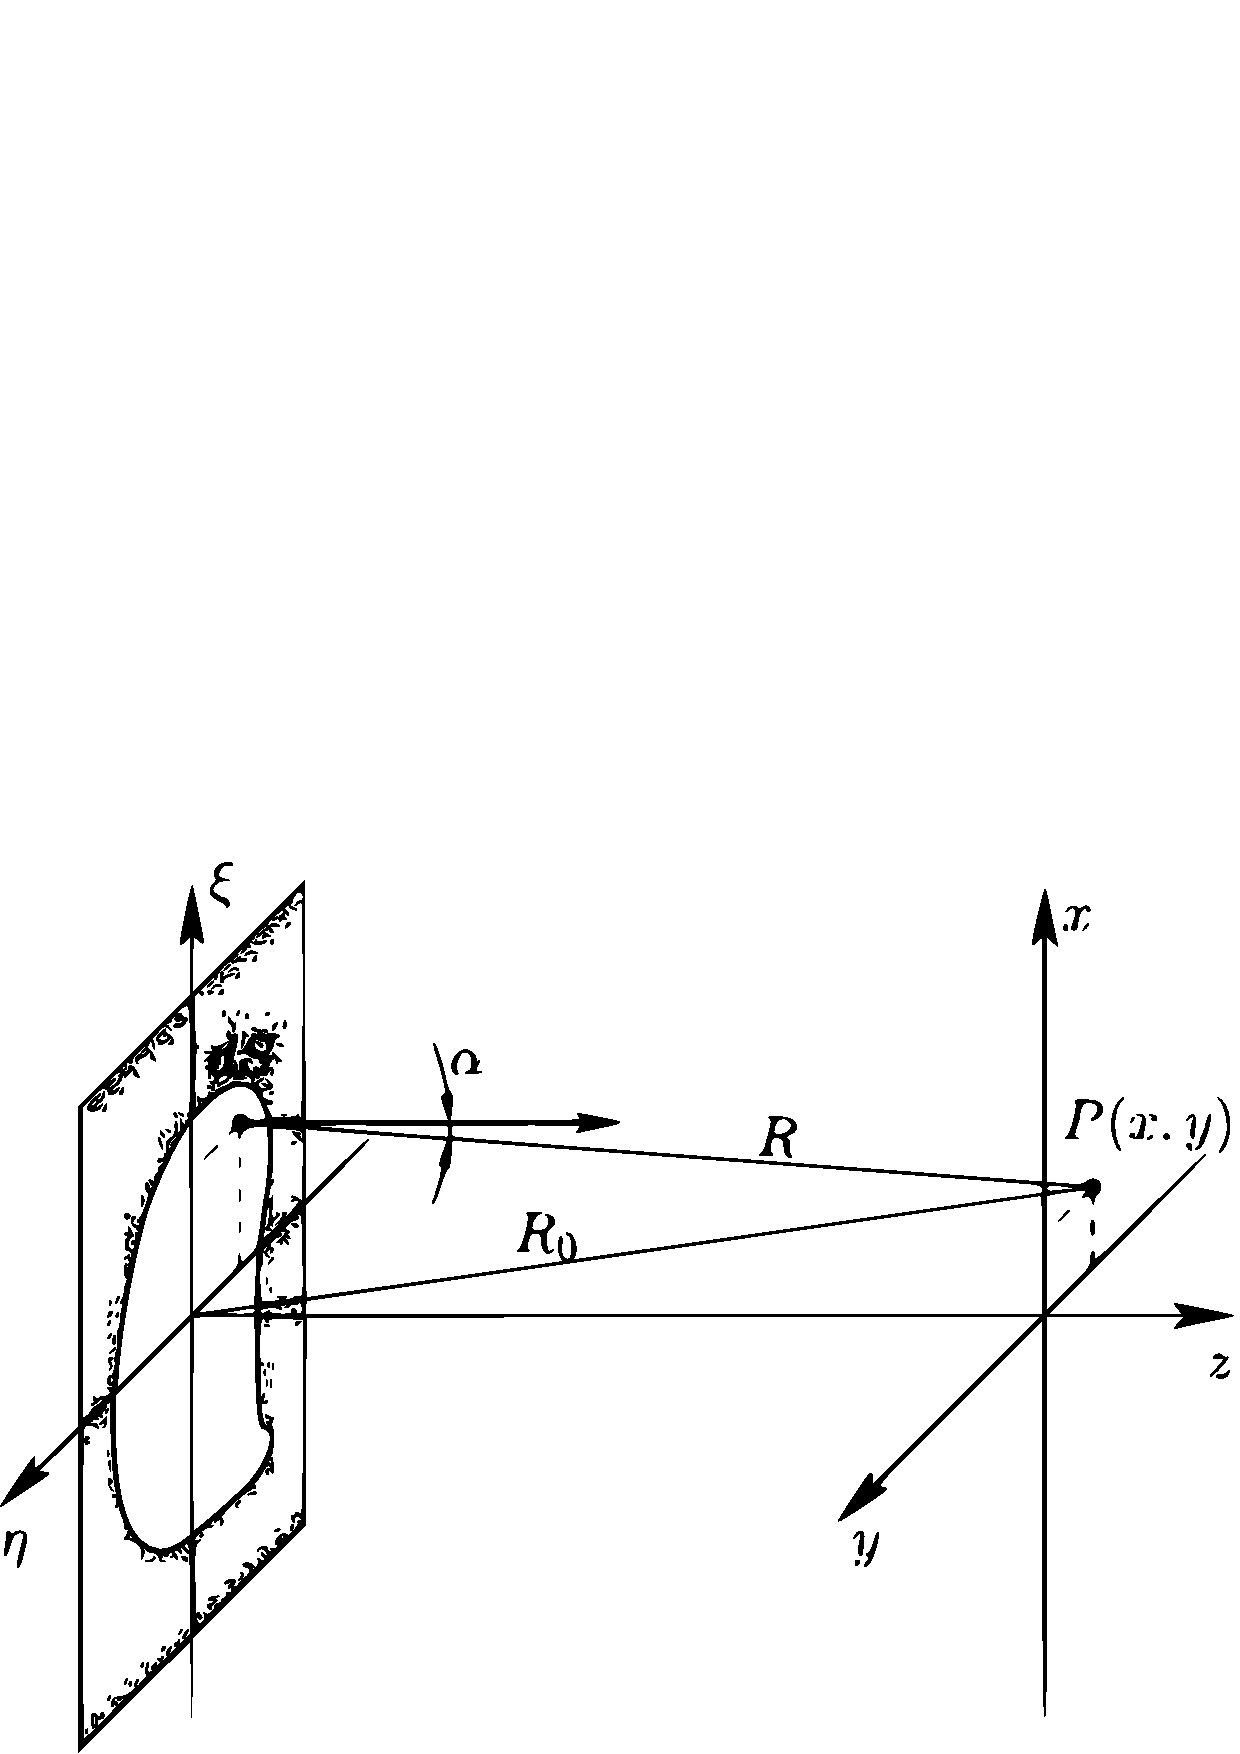
\includegraphics[width = 0.75\textwidth]{images/theory_huygens_frenel.jpg}
                \caption{Полное световое колебание в точке P}
            \end{figure}
    \end{frame}

    \begin{frame}{Теория. Принцип Гюйгенса-Френеля}    
            Полное световое колебание $g(x,y)$ в некоторой точке P:
            \begin{equation}
                g(x,y) = \frac{1}{i\lambda}\iint\limits_{S}f_0(\xi,\eta)\frac{e^{ikR}}{R}cos(\alpha) d\xi d\eta
            \end{equation}
            \begin{itemize}
                \item амплитуда и фаза излучения вторичного источника $\sim$ амплитуде и фазе $a_0(\xi, \eta)$ и $\phi_0(\xi, \eta)$ реальной волны
                \item затенённые участки не переизлучают
                \item в области отверстия волна не искажается
                \item площадка $ds$ переизлучает сферическую волну $\Rightarrow t(x,y) = \frac{1}{R}e^{ikR}$
                \item амплитуда колебания $\sim$ видимой площади $ds$, т.е. $ds \cdot cos\alpha$
                \item $\frac{1}{i\lambda}$ -- нормировочный коэффициент
            \end{itemize}
    \end{frame}

    \begin{frame}{Теория. Френелевское приближение}
        Если предположить, что
        \begin{itemize}
            \item $b \ll R_0$, где $R_0$ -- расстояние до точки наблюдения
            \item $cos\alpha \approx 1$
        \end{itemize}
        принцип Гюйгенса-Френеля запишется в виде:
        \begin{equation}
            g(x,y) = \frac{1}{i\lambda R_0}\iint\limits_{S}f_0(\xi,\eta)e^{ikR}d\xi d\eta
        \end{equation}
        Точное значение $R = z\sqrt{1 + \frac{(x-\xi)^2}{z} + \frac{(y-\eta)^2}{z}}$. Во \textbf{френелевском приближении} ошибка при вычислении фазы колебаний $\Delta(kR) \ll \pi \Rightarrow \Delta R \ll \frac{\lambda}{2}$. Значит 
        \begin{equation}
            R \approx z + \frac{(x-\xi)^2}{2z} + \frac{(y-\eta)^2}{2z}
        \end{equation}
         
    \end{frame}

    \begin{frame}{Теория. Френелевское приближение}
        Таким образом, получим
        \begin{equation}
            g(x,y) = \frac{e^{ikz}}{i\lambda z}\iint f_0(\xi,\eta)e^{i\frac{k}{2z} \left[ (x-\xi)^2 + (y - \eta)^2 \right] }d\xi d\eta
        \end{equation}
        Если отверстие освещается плоской волной амплитуды $A_0$: $f_0(\xi, \eta) \equiv A_0$, а точка наблюдения лежит на оси $z (x=0, y=0)$, то
        \begin{equation}
            g(x,y) = A_0\frac{e^{ikz}}{i\lambda z}\iint e^{i\frac{k}{2z} (\xi^2 + \eta^2) }d\xi d\eta
        \end{equation}
    \end{frame}

    \begin{frame}{Теория. Дифракция Френеля на щели}
        \begin{columns}
            \column{0.4\textwidth}
            \begin{figure}[H]
            \centering
                \includegraphics[width = 0.8\textwidth]{images/theory_fresnel_slit.png}
                \caption{К расчёту дифракции на щели}
            \end{figure}

            \column{0.6\textwidth}
            Световое колебание плоской волны амплитуды $A_0$ равно
            \begin{equation}
                g = A_0\int_{b_1}^{b_2}e^{\frac{ik}{2z}\xi^2}d\xi
            \end{equation}

            Воспользуемся методом векторных диаграмм для расчёта светового поля. Вклад полоски шириной $d\xi$ в колебание в точке P обозначим вектором длины $d\xi$ с углом наклона $\phi = \frac{k}{2z}\xi^2$. Разность фаз между полосками на расстоянии $\xi$ и $\xi+d\xi$ равен 
            \begin{equation}
                d\phi=\frac{k}{z}\xi d\xi
            \end{equation}
        \end{columns}
    \end{frame}

    \begin{frame}{Теория. Дифракция Френеля на щели}
        \begin{columns}
            \column{0.4\textwidth}
            \begin{figure}[H]
                \centering
                \includegraphics[width = 0.8\textwidth]{images/theory_schuster_zone.jpg}
                \caption{Две зоны Шустера}
            \end{figure}
            \column{0.6\textwidth}
                \textbf{Зона Френеля} - зона кольцевой формы
                \textbf{Зона Шустера} - зона в виде полос
                \begin{itemize}
                    \item первый вектор $\Vec{a_0}$ горизонтален
                    \item вектор, отстоящий на $\pi$, противоположен $\Vec{a_0}$. А значит фаза $\frac{k}{2z}\xi_1^2 = \pi \Rightarrow \xi_1 = \sqrt{\lambda z}$ 
                    \item вектор, отстоящий на $2\pi$, сонаправлен с $a_0$, аналогично $\xi_2 = \sqrt{2\lambda z}$
                    \item внешний край $m$-й зоны Шустера отстоит от оси $\eta$ на расстояние $\mathbf{\xi_m = \sqrt{m\lambda z}}$
                    \item $|A_2|$ -- вклад в амплитуду колебаний 2-й зоны шустера.
                \end{itemize}
        \end{columns}
    \end{frame}

    \begin{frame}{Теория. Дифракция Френеля на щели}
        \begin{columns}
            \column{0.3\textwidth}
            \begin{figure}[H]
                \centering
                \includegraphics[width = 0.8\textwidth]{images/theory_1t_exp.jpg}
                \caption{Зоны Шустера в плоскости щели}
            \end{figure}
            
            \column{0.7\textwidth}
                Вид наблюдаемой дифракционной картины на щели $b$ определяется \textit{волновым парметром}:
                \begin{equation}
                    p = \frac{\sqrt{z\lambda}}{b}
                \end{equation}
                Также используют \textbf{чило Френеля}: $C = \frac{b^2}{z\lambda} = \frac{1}{p^2}$, равное полному числу открытых зон Френеля на всей ширине щели.\\
                \begin{itemize}
                    \item если $p \sim 1$ -- область дифракции Френеля (\textit{ближняя волновая зона})
                    \item если число зон Френеля, укладывающихся на полуширине щели $b/2$, равно $m$, то наблюдается $n = m - 1$ тёмных полос.
                \end{itemize}
        \end{columns}
    \end{frame}

    \begin{frame}{Экспериментальная установка}
    \small
    \begin{figure}[H]
        \centering
        \includegraphics[width = \textwidth]{images/a.pdf}
        \caption{Схема установки для наблюдения дифракции Френеля}
        \label{fig:inst_a}
    \end{figure}
	\end{frame}
    
    \begin{frame}{Измерения и обработка результатов}
         \begin{columns}
            \column{0.5\textwidth}
            \begin{figure}[H]
            \centering
                \includegraphics[width = \textwidth]{images/graph_a.png}
                \caption{Зависимость расстояния до щели $z$ от $1/m$}
            \end{figure}

            \column{0.5\textwidth}
            \begin{itemize}
                \item $2 \xi = \frac{\sqrt{z}}{\sqrt{\frac{1}{n}}} \cdot \sqrt{\lambda} = \left( 0.326 \pm 0.003 \right) \text{ мм}$ -- ширина щели, полученная из графика
                \item $b = \left( 0.321 \pm 0.001 \right) \text{ мм}$ -- ширина щели, измеренная с помощью микрометрического винта
            \end{itemize}
        \end{columns}
    \end{frame}

    \section{Дифракция Фраунгофера на щели}

    \begin{frame}{Теория. Дифракция Фраунгофера на щели}
        Рассмотрим дифракцию на отверстии, находящемся в плоскости $z=0$.
        \begin{itemize}
            \item $R = \sqrt{z^2+(x-\xi)^2+(y-\eta)^2} = \sqrt{R_0 - (2x\xi+2y\eta)+(\xi^2+\eta^2)}$
            \item $R \approx R_0 - \frac{x\xi + y\eta}{R_0} + \frac{\xi^2 + \eta^2}{2R_0}$
            \item пусть максимальный размер отверстия $b^2 \geq \eta^2 + \xi^2$
            \item точка P удалена настолько, что выполняется $\frac{b^2}{R_0} \ll \lambda$
        \end{itemize}
        Тогда $R \approx R_0 - \frac{x\xi}{R_0} - \frac{y\eta}{R_0}$ и введём $u = \frac{kx}{R_0}, v = \frac{ky}{R_0}$. В этом приближении принцип Гюйгенса-Френеля имеет вид
        \begin{equation}
            g(u,v) = \frac{e^ikR_0}{i\lambda R_0}\iint f_0(\xi, \eta)e^{-i(u\xi + v\eta)}d\xi d\eta
        \end{equation}
        $g(u,v)$ - \textbf{двумерное преобразование Фурье} граничного поля $f_0(x,y)$ в плоскости наблюдения.
    \end{frame}

    \begin{frame}{Теория. Дифракция Фраунгофера на щели}
        В одномерном случае (щель) 
        \begin{equation}
            g(u) \sim \int_{-\infty}^{+\infty}f_0(\xi)e^{-ik\xi sin\theta}d\xi \sim \frac{sin(\frac{kb}{2}sin\theta)}{\frac{kb}{2}sin\theta},
        \end{equation}
        где $sin\theta = \frac{x}{R_0}$. Вторичные волны, приходящие в точку наблюдения, можно считать параллельными. \\
        Интенсивность $I(\theta) = |g(\theta)|^2$ обращается в 0 (тёмные полосы) при $\frac{kb}{2}sin\theta = m\pi$ откуда 
        \begin{equation}
            sin\theta = m\frac{\lambda}{b}
        \end{equation}
        Расстояние от тёмной полосы до оптической оси объектива $x_m = m\frac{\lambda}{b}f_2$, где $f_2$ - фокусное расстояние объектива $O_2$
    \end{frame}

    \begin{frame}{Экспериментальная установка}
        \begin{figure}[H]
            \centering
            \includegraphics[width = \textwidth]{images/b.pdf}
            \caption{Схема установки для наблюдения дифракции Фраунгофера на щели}
            \label{fig:inst_b}
        \end{figure}
    \end{frame}

    \begin{frame}{Измерения и обработка результатов}
       \begin{columns}
            \column{0.5\textwidth}
            \begin{figure}[H]
            \centering
                \includegraphics[width = \textwidth]{images/graph_b.png}
                \caption{Зависимость положений экстремумов дифракционной картины от их номера}
            \end{figure}

            \column{0.5\textwidth}
            \begin{itemize}
                \item $\Delta X = \left( 0.17 \pm 0.01 \right) \text{мм}$ -- расстояние между полосами (угол наклона);
                \item $b = \frac{\lambda}{\Delta X} f_2 = \left( 0.34 \pm 0.01 \right) \text{ мм}$ -- измерение ширины щели по наклону прямой;
                \item $b = \left( 0.363 \pm 0.001 \right)\text{ мм}$ -- измерение ширины щели с помощью микрометрического винта.
            \end{itemize}
        \end{columns}
    \end{frame}

    \section{Дифракция Фраунгофера на двух щелях}
    \begin{frame}{Теория. Дифракция Фраунгофера на двух щелях}
        \begin{columns}
            \column{0.3\textwidth}
            \begin{figure}[H]
                \centering
                \includegraphics[width = 0.8\textwidth]{images/thoery_two_slit.jpg}
                \caption{Разность хода при двух щелях}
            \end{figure}
            \begin{figure}[H]
                \centering
                \includegraphics[width = 0.8\textwidth]{images/theory_two_slit_destr.jpg}
                \caption{Разность хода при двух щелях}
            \end{figure}
            
            \column{0.7\textwidth}
                \begin{itemize}
                    \item $\Delta =dsin\theta$
                    \item фаза отличается на величину $\alpha = -k\Delta = -kdsin\theta$
                    \item функция колебательного процесса от второй щели $g(\theta)e^{i\alpha}$
                    \item амлитуда суммарного колебательного процесса $g(\theta) + g(\theta)e^{i\alpha}$
                    \item угловая координата интерфернционного максимума $m$-ого порядка $\theta_m = m\frac{\lambda}{d}$
                    \item линейное расстояние между соседними интерференционными полосами $\delta x = f_2\frac{\lambda}{d}$
                    \item число интерференционных полос в центральной области $n = \frac{2\lambda f_2}{b} \frac{1}{\delta x} = \frac{2d}{b}$
                \end{itemize}
        \end{columns}
    \end{frame}

     \begin{frame}{Экспериментальная установка}
      \begin{figure}[H]
          \centering
          \includegraphics[width = \textwidth]{images/c.pdf}
          \caption{Схема для наблюдения дифракции Фраунгофера на двух щелях}
          \label{fig:inst_c}
      \end{figure}
    \end{frame}
   

    \begin{frame}{Измерения и обработка результатов}
     \begin{columns}
     
            \column{0.3\textwidth}
            \begin{figure}[H]
            \centering
                \includegraphics[width = \textwidth]{images/photo_3.jpg}
                \caption{Дифракционная картина на двух щелях}
            \end{figure}

            \column{0.7\textwidth}
            \begin{itemize}
                \item $\delta x = \frac{ \left( 0.38 \pm 0.02 \right) \text{ мм}}{6} = \left( 0.063 \pm 0.003 \right) \text{ мм}$ -- измеренное расстояние между дифракционными минимумами
                \item $d = f_2 \frac{\lambda}{\delta x} = \left( 0.94 \pm 0.04 \right) \text{ мм}$ -- расстояние между щелями
                \item $b = \frac{2d}{n} = \left( 0.31 \pm 0.01 \right) \text{ мм}$ -- ширина входной щели
        \end{itemize}
        
        \end{columns}
    \end{frame}

   \begin{frame}{Измерение размеров двойной щели}
   \begin{columns}
 
        \column{0.4\textwidth}
        \begin{figure}[H]
        \centering
            \includegraphics[width = \textwidth]{images/slit.png}
            \caption{Изображение щелей в микроскопе}
        \end{figure}

        \column{0.6\textwidth}
        \begin{itemize}
            \item $d = \left( 0.94 \pm 0.02 \right) \text{ мм}$ -- расстояние между щелями
            \item $D_1 = \left( 0.18 \pm 0.02 \right) \text{ мм}$ -- длина первой щели
            \item $D_2 = \left( 0.20 \pm 0.02 \right) \text{ мм}$ -- длина первой щели
        \end{itemize}
        
        \end{columns}
   \end{frame}
   
    \section{Влияние на разрешающую способность оптического инструмента}
    \begin{frame}{Теория. Влияние дифракции на оптические приборы}
    \begin{itemize}
        \item расстояние между изображениями щелей в плоскости П равно $l = \phi f_2 = d \frac{f_2}{f_1}$
        \item ширина каждого изображения $\delta x \approx \frac{\lambda}{b}f_2$ определяется дифракцией света на щели $S_2$.
        \item когда $\frac{\delta x}{2} \ge l$, то по виду двойная $\approx$ одиночная щель
        \item \textbf{критерий Рэлея}: когда $\delta x \sim l$ или $\frac{\lambda}{b} \sim \frac{d}{f_1}$, то изображения различны
    \end{itemize}
    \end{frame}

   \begin{frame}{Экспериментальная установка}
      \begin{figure}[H]
          \centering
          \includegraphics[width = \textwidth]{images/d.pdf}
          \caption{Схема для исследования разрешающей способности оптического инструмента}
          \label{fig:inst_d}
      \end{figure}
   \end{frame}

   \begin{frame}{Измерения и обработка результатов}
        Для проверки справедливости критерия Рэлея сравнили измеренную ширину $b_0$ щели $S_2$, при которой изображение двух щелей сливается, но все ещё различимо, с расчётом по формуле, приведённой на предыдущем слайде.

        \begin{itemize}
            \item $b_0^{exp} = \left( 0.181 \pm 0.001 \right) \text{ мм}$ -- измеренная ширина щели
            \item $b_0^{theor} > 0.077 \text{ мм}$ -- критическая ширина щели, при которой пятна от двух щелей сольются в одно
        \end{itemize}
   \end{frame}

\section{Заключение. Выводы}
    \begin{frame}{Заключение}
        \begin{itemize}
            \item при рассмотрении \textit{дифракции Френеля} было измерено значение ширины щели двумя способами. Результаты измерений различаются на 1.5\%
            \item при исследовании \textit{дифракции Френеля} на тонкой вертикальной нити, при удалении микроскопа от нити, на её фоне всегда наблюдается чётное число тёмных дифракционных полос
            \item при рассмотрении \textit{дифракции Фраунгофера на щели} значения ширины щели, измеренные по формуле и по микроскопическому винту, различаются не более, чем на 5\%
            \item при рассмотрении \textit{дифракции Фраунгофера на двух щелях} непосредственное расстояние между щелями $d$ совпадают с вычислениями
            \item при изучении \textit{влияния дифракции на разрешающую способность оптического инструмента} получили, что $b_0 > \lambda f_1 /d$, что означает разрешимость изображений по Рэлею
        \end{itemize}
    \end{frame}
    
\end{document}